% Provenance (never printed): old terminale S material on the continental crust
% (granitic composition, thickness, density, age; roots and isostasy). Thickness
% from Christensen-Mooney 1995 and Cogley 1984 (CRUST1.0 dropped: no licence,
% Sync 1); ocean-floor ages from figdata/grade-12/crust_ages.py (Seton 2020 grid,
% as in g11.01). Airy isostasy is g11.03's: recalled, not re-derived. Radiometric
% dating is g12.07's: ages are only quoted here.
\chapter{La croûte continentale}\label{ch:g12:continental-crust}

Dans le nord-ouest du Canada, près de la rivière Acasta, affleure une roche
grise striée de bandes claires et sombres. Elle a été datée de 4.00 à
4.03~milliards d'années~: c'est le gneiss d'Acasta, la plus ancienne roche
connue. Plus anciens encore sont des grains d'un minéral, le zircon, longs
chacun d'une fraction de millimètre, trouvés dans de vieilles roches
sédimentaires des Jack Hills, en Australie-Occidentale. Arrachés à des
roches plus anciennes et transportés par l'eau avant d'être enfouis, ils
ont cristallisé il y a 4.4~milliards d'années, et ils montrent qu'une croûte
existait déjà. Aucun fond océanique n'a même le vingtième de cet âge. Ce
chapitre cherche de quoi sont faits les continents, et pourquoi ils durent.
% ledger: bowring99:acasta, wilde01:zircon, uw14:jack-hills, photo:g12-acasta, photo:g12-jack-hills-zircons

\begin{omfigure}
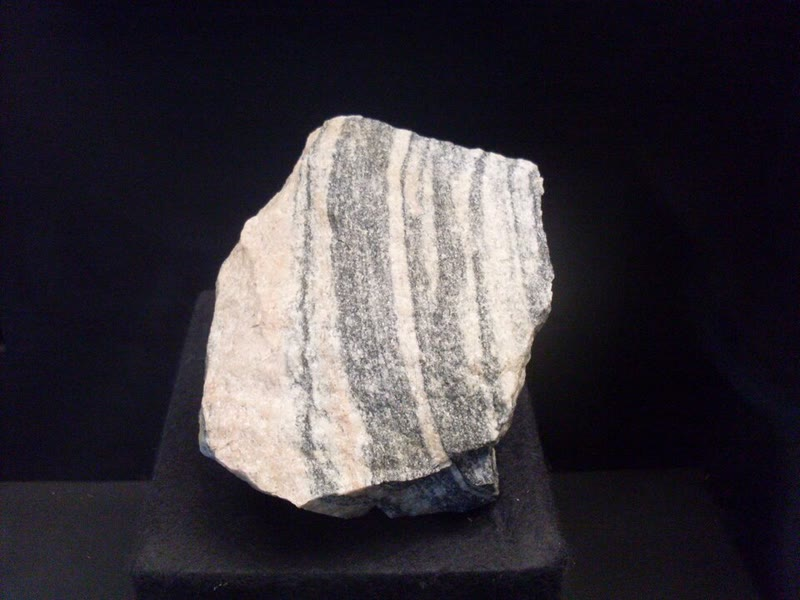
\includegraphics[height=4.6cm]{images/book2/g12-pedro-acasta-gneiss.jpg}\hspace{0.04\linewidth}%
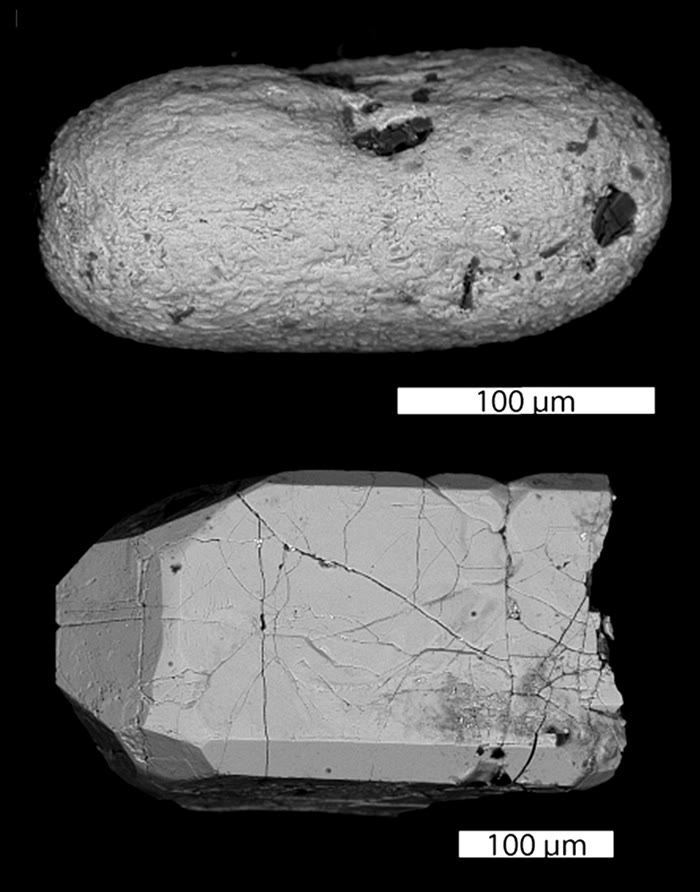
\includegraphics[height=4.6cm]{images/book2/g12-cavosie-jack-hills-zircons.jpg}

{\small À gauche~: un fragment du gneiss d'Acasta, vieux de 4.03~milliards
d'années, dans une vitrine de musée. Photographie Pedroalexandrade
(CC~BY-SA~3.0). À droite~: deux grains de zircon des Jack Hills, en
Australie-Occidentale, vus au microscope électronique~; chaque barre
d'échelle mesure \qty{100}{\micro m}. Le grain du haut a été arrondi
pendant son transport par l'eau, celui du bas a gardé ses faces cristallines.
Images A.~Cavosie et J.~Valley (domaine public).}
\end{omfigure}
% ledger: photo:g12-acasta, photo:g12-jack-hills-zircons

\begin{recall}
La croûte s'arrête au \omterm{def:g11:seismic-structure:moho}{Moho}, sous lequel se trouve le manteau, plus dense
(\cref{ch:g11:seismic-structure}). La \omterm{def:g11:ocean-ridges:oceanic-lithosphere}{croûte océanique} est formée d'environ
\qty{7}{km} de basalte et de \omterm{def:g11:ocean-ridges:gabbro}{gabbro} fabriqués aux dorsales
(\cref{ch:g11:ocean-ridges}), et elle n'a jamais plus de 190 millions
d'années environ (\cref{ch:g11:drift-to-spreading}). Les couches
superficielles flottent sur l'\omterm{def:g11:lithosphere-asthenosphere:lithosphere}{asthénosphère}~: dans le modèle d'Airy, une
région plus haute d'une hauteur $h$ a une croûte plus épaisse de $h\,\rho_m/(\rho_m -
\rho_c)$ (\cref{ch:g11:lithosphere-asthenosphere}). Les
roches magmatiques sont nommées d'après leur \omterm{def:g11:igneous-rocks:texture}{texture} et leur teneur en
silice~: \omterm{def:g11:igneous-rocks:felsic-mafic}{mafiques} de 45 à \qty{55}{\percent} de \ce{SiO2}, \omterm{def:g11:igneous-rocks:felsic-mafic}{intermédiaires} de
55 à 65, \omterm{def:g11:igneous-rocks:felsic-mafic}{felsiques} de 65 à 75 (\cref{ch:g11:igneous-rocks}). Les éléments
radioactifs se désintègrent à un rythme constant, ce qui donne leur âge aux
roches (les livres de physique~; \cref{ch:g12:age-of-the-earth}).
\end{recall}
% ledger: white92:crust, data:b2-seafloor-age, tulane:magma-types

\section{De quoi sont faits les continents}

\begin{definition}[Croûte continentale]\label{def:g12:continental-crust:continental-crust}
La \emph{croûte continentale}\index{croute continentale@croûte continentale}
est la croûte qui forme les continents, y compris leurs parties situées sous
des mers peu profondes. Elle est épaisse, de composition granitique en
moyenne dans sa partie supérieure, légère, et elle peut être très ancienne.
\end{definition}
% ledger: tulane:crust-types, tulane:roots, cogley84:continents

Les continents sont plus grands que les terres émergées. Les bords de la
\omterm{def:g12:continental-crust:continental-crust}{croûte continentale} se trouvent sous la mer, sur les plateaux
continentaux~: cartographiée ainsi, la \omterm{def:g12:continental-crust:continental-crust}{croûte continentale} couvre
\num{210}~millions de~\unit{km^2}, soit \qty{41}{\percent} de la surface de
la Terre, dont près d'un tiers, \qty{30.6}{\percent}, est immergé. Comptée
avec ses parties immergées, l'altitude moyenne de la \omterm{def:g12:continental-crust:continental-crust}{croûte continentale}
n'est que d'environ \qty{120}{m} au-dessus du niveau de la mer.
% ledger: cogley84:continents

En surface, les continents montrent toutes sortes de roches --- sédiments,
\omterm{def:g11:igneous-rocks:volcanic-plutonic}{roches volcaniques}, roches métamorphiques ---, mais sous la couverture
sédimentaire, la \omterm{def:g12:continental-crust:continental-crust}{croûte continentale} est faite surtout de roches
granitiques et des roches métamorphiques et \omterm{def:g11:igneous-rocks:volcanic-plutonic}{plutoniques} d'anciennes \omterm{def:g12:continental-crust:root}{racines}
de montagnes. En moyenne, l'ensemble de la \omterm{def:g12:continental-crust:continental-crust}{croûte continentale} contient
\qty{60.6}{\percent} de silice~; sa partie supérieure en est plus riche,
\qty{66.6}{\percent}, si bien que sa partie profonde doit en être plus
pauvre.
% ledger: rg14:crust, tulane:crust-types, cm95:crust

\begin{omfigure}
\begin{tikzpicture}
\begin{axis}[omrecord, ybar=0pt, width=0.92\linewidth, height=5.0cm, bar width=7pt,
  ymin=0, ymax=80, ylabel={fraction massique (\unit{\percent})},
  symbolic x coords={SiO2, Al2O3, FeO, MgO, CaO, Na2O, K2O},
  xticklabels={\ce{SiO2}, \ce{Al2O3}, \ce{FeO}, \ce{MgO}, \ce{CaO}, \ce{Na2O}, \ce{K2O}},
  xtick=data, enlarge x limits=0.08, ymajorgrids=true, xmajorgrids=false,
  legend style={font=\scriptsize, at={(0.98,0.97)}, anchor=north east, legend columns=1}]
% ledger: rg14:crust (upper and bulk continental crust; FeO* total iron)
\addplot[fill=omLithGranite, draw=black!60] coordinates {(SiO2,66.6) (Al2O3,15.4) (FeO,5.04) (MgO,2.48) (CaO,3.59) (Na2O,3.27) (K2O,2.80)};
\addplot[fill=omProp!55, draw=black!60] coordinates {(SiO2,60.6) (Al2O3,15.9) (FeO,6.71) (MgO,4.66) (CaO,6.41) (Na2O,3.07) (K2O,1.81)};
% ledger: earle:magma-oxides (mafic magma: midpoint of each range, the bar spans the range)
\addplot[fill=omLithBasalt, draw=black!60, error bars/.cd, y dir=both, y explicit]
  coordinates {(SiO2,50) +- (0,5) (Al2O3,16) +- (0,2) (FeO,10) +- (0,2) (MgO,7) +- (0,2) (CaO,9) +- (0,2) (Na2O,2) +- (0,1) (K2O,1.75) +- (0,1.25)};
\legend{croûte continentale supérieure, croûte continentale entière, magma mafique (intervalle)}
\end{axis}
\end{tikzpicture}

{\small Composition de la \omterm{def:g12:continental-crust:continental-crust}{croûte continentale} comparée à celle d'un magma
\omterm{def:g11:igneous-rocks:felsic-mafic}{mafique}, celui qui forme la \omterm{def:g11:ocean-ridges:oceanic-lithosphere}{croûte océanique}~: les principaux oxydes, en
pourcentage de la masse (\ce{FeO} compte tout le fer). La \omterm{def:g12:continental-crust:continental-crust}{croûte
continentale} est plus riche en silice, en sodium et en potassium, plus
pauvre en fer, en magnésium et en calcium. Données~: Rudnick et Gao
(2014)~; intervalle \omterm{def:g11:igneous-rocks:felsic-mafic}{mafique} d'après S.~Earle, \emph{Physical Geology}
(CC~BY~4.0).}
\end{omfigure}
% ledger: rg14:crust, earle:magma-oxides

\section{Une croûte épaisse et légère}

Les campagnes sismiques trouvent le \omterm{def:g11:seismic-structure:moho}{Moho} sous les continents à des
profondeurs très différentes. En moyenne sur tous les continents, pondérée
par la surface, la croûte est épaisse d'environ \qty{41}{km}~; elle est
plus mince, environ \qty{30}{km}, là où elle a été étirée, et plus épaisse,
environ \qty{46}{km} en moyenne, dans les chaînes de montagnes. Loin des
chaînes, elle est couramment épaisse de 35 à \qty{40}{km}~; sous les plus
hautes chaînes, de 50 à \qty{70}{km}, environ \qty{70}{km} sous certaines
parties du Tibet. La \omterm{def:g11:ocean-ridges:oceanic-lithosphere}{croûte océanique} est épaisse d'environ \qty{7}{km}~:
la \omterm{def:g12:continental-crust:continental-crust}{croûte continentale} est cinq à dix fois plus épaisse.
% ledger: cm95:crust, tulane:roots, karplus:tibet-moho, white92:crust

\begin{omfigure}
\begin{tikzpicture}
\begin{axis}[omrecord, xbar, bar shift=0pt, width=0.78\linewidth, height=5.0cm, bar width=8pt,
  xmin=0, xmax=80, ymin=0.4, ymax=5.6, ytick={1,...,5},
  yticklabels={croûte océanique, continents étirés, continents (moyenne), montagnes (moyenne), sous le Tibet},
  xlabel={épaisseur de la croûte (\unit{km})}, ymajorgrids=false,
  nodes near coords, nodes near coords style={font=\scriptsize, anchor=west}, point meta=explicit symbolic]
% ledger: white92:crust, cm95:crust, karplus:tibet-moho
\addplot[fill=omLithBasalt, draw=black!60] coordinates {(7.1,1) [7.1]};
\addplot[fill=omLithGranite, draw=black!60] coordinates {(30.5,2) [30.5] (41.1,3) [41.1] (46.3,4) [46.3] (70,5) [environ 70]};
\end{axis}
\end{tikzpicture}

{\small Épaisseur de la croûte d'après les mesures sismiques. Données~:
White, McKenzie et O'Nions (1992) pour la \omterm{def:g11:ocean-ridges:oceanic-lithosphere}{croûte océanique}~; Christensen et
Mooney (1995) pour les moyennes continentales~; Karplus et ses collègues
(2019) pour le Tibet.}
\end{omfigure}
% ledger: white92:crust, cm95:crust, karplus:tibet-moho

La \omterm{def:g12:continental-crust:continental-crust}{croûte continentale} est aussi légère. Sa masse volumique moyenne est
d'environ \qty{2830}{kg/m^3}. Le basalte et le \omterm{def:g11:ocean-ridges:gabbro}{gabbro} de la \omterm{def:g11:ocean-ridges:oceanic-lithosphere}{croûte
océanique}, riches en pyroxène et en olivine, atteignent environ
\qty{3000}{kg/m^3} (\cref{ch:g11:minerals}), et le manteau situé juste sous
le \omterm{def:g11:seismic-structure:moho}{Moho} environ \qty{3380}{kg/m^3}. Une croûte épaisse et légère flotte
haut~: c'est pourquoi les continents se dressent au-dessus du fond des
océans, et pourquoi un continent ne peut pas être entraîné vers le bas dans
une \omterm{def:g11:subduction-zones:subduction}{zone de subduction}. Là où un continent arrive à une fosse, il est trop
léger pour s'enfoncer~; la \omterm{def:g11:subduction-zones:subduction}{subduction} s'arrête, et les deux continents
entrent en collision (\cref{ch:g12:mountain-building}). Une fois formée, la
\omterm{def:g12:continental-crust:continental-crust}{croûte continentale} est difficile à détruire.
% ledger: cm95:crust, data:prem, tulane:roots, tulane:no-subduct
% values (mineral_density.py): basalt/gabbro rock line 3.0015 g/cm3

\begin{omfigure}
\begin{tikzpicture}[x=1cm, y=0.075cm, font=\footnotesize]
  % continental column: 41 km of crust, surface at +0.12 km (mean height); ocean column: 3.7 km of water drawn schematically
  \fill[omLithGranite] (0,0) rectangle (3,-41);
  \fill[omLithPeridotite!60] (0,-41) rectangle (3,-60);
  \fill[omSea] (6,0) rectangle (9,-4);
  \fill[omLithGabbro] (6,-4) rectangle (9,-11.1);
  \fill[omLithPeridotite!60] (6,-11.1) rectangle (9,-60);
  \draw[black!60] (0,0) rectangle (3,-60) (6,0) rectangle (9,-60);
  \draw[line width=0.9pt] (0,-41) -- (3,-41) (6,-11.1) -- (9,-11.1);
  \node[align=center] at (1.5,-20) {croûte continentale\\environ \qty{41}{km}\\\qty{2830}{kg/m^3}\\jusqu'à 4 milliards d'années};
  \node[align=center] at (7.5,-24) {manteau\\\qty{3380}{kg/m^3}\\sous le Moho};
  \node[align=center] at (1.5,-50.5) {manteau};
  \node at (7.5,-2) {océan};
  \draw[black!60] (8.6,-7.6) -- (9.3,-7.6);
  \node[anchor=west, align=left] at (9.3,-7.6) {croûte océanique, environ \qty{7}{km}\\\qty{3000}{kg/m^3}\\moins de 200 millions d'années};
  \node[anchor=east] at (-0.1,-41) {Moho};
  \node[anchor=east] at (5.9,-11.1) {Moho};
  \node[anchor=south] at (1.5,0) {un continent};
  \node[anchor=south] at (7.5,0) {un océan};
  \foreach \d in {0,20,40,60} {\draw[black!60] (-1.5,-\d) -- (-1.3,-\d); \node[anchor=east, font=\scriptsize] at (-1.5,-\d) {\d};}
  \draw[black!60] (-1.4,0) -- (-1.4,-60);
  \node[rotate=90, font=\scriptsize] at (-2.3,-30) {profondeur (\unit{km})};
\end{tikzpicture}

{\small Un continent et un océan côte à côte (profondeurs à l'échelle,
largeurs non~; l'océan est dessiné profond de \qty{4}{km})~: la \omterm{def:g12:continental-crust:continental-crust}{croûte
continentale} est plus épaisse, plus légère et beaucoup plus ancienne que la
\omterm{def:g11:ocean-ridges:oceanic-lithosphere}{croûte océanique}.}
\end{omfigure}
% ledger: cm95:crust, white92:crust, data:prem, bowring99:acasta, data:b2-seafloor-age

\begin{method}[Comparer la croûte continentale et la croûte océanique]\label{met:g12:continental-crust:compare}
Pour savoir quel type de croûte se trouve sous un lieu, comparer cinq
propriétés~:
\begin{enumerate}
  \item l'épaisseur~: environ \qty{7}{km} pour la \omterm{def:g11:ocean-ridges:oceanic-lithosphere}{croûte océanique}, de 30 à
        \qty{70}{km} pour la \omterm{def:g12:continental-crust:continental-crust}{croûte continentale}~;
  \item les roches~: basalte et \omterm{def:g11:ocean-ridges:gabbro}{gabbro}, ou granite, gneiss et roches
        apparentées, sous une couverture de sédiments~;
  \item la composition~: environ \qty{50}{\percent} de silice, ou environ
        60 et plus~;
  \item la masse volumique~: environ \qty{3000}{kg/m^3}, ou environ
        \qty{2830}{kg/m^3}~;
  \item l'âge~: moins de 200 millions d'années, ou jusqu'à 4 milliards
        d'années.
\end{enumerate}
L'altitude est un indice, pas un critère~: la plus grande partie du fond
des océans se trouve à des kilomètres de profondeur, mais les bords des
continents sont sous des mers peu profondes.
\end{method}
% ledger: white92:crust, cm95:crust, rg14:crust, earle:magma-oxides, cogley84:continents

\begin{example}[Un fond marin peu profond]\label{ex:g12:continental-crust:shelf}
Un navire océanographique trouve un fond marin à \qty{150}{m} de
profondeur. Les profils sismiques placent le \omterm{def:g11:seismic-structure:moho}{Moho} \qty{32}{km} sous le
fond~; une carotte de forage remonte, sous les sédiments, une roche à gros
grains faite de quartz, de feldspath et de mica. Quelle croûte se trouve
là~?

\emph{Solution.} Une épaisseur d'environ \qty{32}{km}~: continentale, plus
mince que la moyenne, comme là où elle a été étirée. Un granite sous les
sédiments~: continentale. Le fond marin est un plateau continental, l'une
des parties immergées qui forment près d'un tiers des continents.
\end{example}
% invented numbers; ledger: cm95:crust, cogley84:continents

Quelle est la masse de toute cette croûte~? Une couche mince devant le
rayon de la Terre a une masse simple à calculer.

\begin{proposition}[La masse d'une couche mince]\label{prop:g12:continental-crust:thin-layer}
Une couche d'épaisseur $H$ et de masse volumique $\rho$ qui couvre une
fraction $f$ de la surface d'une planète de rayon $R \gg H$ et de masse
volumique moyenne $\bar\rho$ a une masse $m \approx 4\pi R^2 f H \rho$, et
sa part dans la masse $M$ de la planète vaut
\[
  \frac{m}{M} \approx 3 f\,\frac{H}{R}\,\frac{\rho}{\bar\rho}.
\]
\end{proposition}
% ledger: earth:Rmean, earth:density

\begin{proof}
La surface de la planète vaut $4\pi R^2$~; la couche en couvre
$4\pi R^2 f$ et, étant mince, a un volume proche de cette aire multipliée
par $H$, donc $m \approx 4\pi R^2
f H \rho$. La masse de la planète vaut
$M = \tfrac{4}{3}\pi R^3 \bar\rho$. En divisant,
$m/M \approx 4\pi R^2 f H \rho / (\tfrac{4}{3}\pi R^3 \bar\rho) = 3 f (H/R)
(\rho/\bar\rho)$.
\end{proof}

Pour la \omterm{def:g11:ocean-ridges:oceanic-lithosphere}{croûte océanique} --- les \qty{59}{\percent} restants de la surface,
\qty{7.1}{km}, environ \qty{3000}{kg/m^3} ---, avec $R = \qty{6371}{km}$ et
$\bar\rho = \qty{5513}{kg/m^3}$, la part vaut $3 \times 0.59 \times
(7.1/6371) \times (3000/5513) \approx 0.0011$~:
environ un millième de la masse de la Terre. Le problème du week-end fait
le même calcul pour les continents.
% ledger: cogley84:continents, white92:crust, earth:Rmean, earth:density

\section{Une croûte ancienne}

Le fond des océans est jeune partout~: les trois quarts ont moins de 100
millions d'années, et presque rien n'a plus de 190 millions d'années. Les
continents, c'est autre chose. Leurs roches couvrent presque toute
l'histoire de la Terre, du gneiss d'Acasta, vieux de 4.03~milliards
d'années, aux laves émises aujourd'hui, et des grains de zircon font
remonter l'archive jusqu'à 4.4~milliards d'années.
% ledger: data:b2-seafloor-age, bowring99:acasta, uw14:jack-hills

\begin{omfigure}
\begin{tikzpicture}
\begin{axis}[omrecord, ybar interval, width=0.82\linewidth, height=5.0cm,
  xmin=0, xmax=200, ymin=0, ymax=0.12, xtick={0,20,...,200},
  xlabel={âge du fond océanique (millions d'années)},
  ylabel={part du fond océanique}, yticklabel style={/pgf/number format/fixed},
  ymajorgrids=true, xmajorgrids=false, clip=false, x tick label as interval=false]
% computed in figdata/grade-12/crust_ages.py (Seton 2020 grid, 1-degree cells, area-weighted)
\addplot[fill=omDef!35, draw=omDef] table[x=age_lo, y=share] {figdata/out/grade-12-crust_ages-hist.dat};
\node[anchor=north east, align=right, font=\scriptsize, fill=white, inner sep=2pt] at (axis cs:198,0.115)
  {plus ancienne roche continentale~: \num{4030} millions d'années,\\vingt fois plus que le plus ancien fond océanique};
\end{axis}
\end{tikzpicture}

{\small L'âge du fond des océans~: la part de sa surface dans chaque
tranche de 10 millions d'années. Le fond jeune domine~; presque rien n'a
plus de 190 millions d'années (quelques vieux bassins de la Méditerranée
orientale sont laissés de côté). Données~: Seton et ses collègues (2020),
calcul.}
\end{omfigure}
% ledger: data:b2-seafloor-age, bowring99:acasta
% values (crust_ages.py): oldest_open_myr 192.5, share_younger_100 0.765, share_younger_150 0.956, rock_over_floor 20.9

Les parties les plus anciennes des continents en forment le cœur.

\begin{definition}[Craton]\label{def:g12:continental-crust:craton}
Un \emph{craton}\index{craton} est un cœur ancien et stable d'un
continent~: une \omterm{def:g12:continental-crust:continental-crust}{croûte continentale} formée et déformée il y a plus d'un
milliard d'années, qui s'est refroidie depuis et ne se déforme plus. Ses
roches sont surtout des roches métamorphiques et \omterm{def:g11:igneous-rocks:volcanic-plutonic}{plutoniques}, les \omterm{def:g12:continental-crust:root}{racines}
profondes d'anciennes montagnes.
\end{definition}
% ledger: tulane:cratons

Autour des \omterm{def:g12:continental-crust:craton}{cratons} s'étendent des ceintures de roches déformées plus
jeunes, les \omterm{def:g12:continental-crust:root}{racines} érodées de chaînes de montagnes édifiées plus tard~;
ces ceintures sont en général de plus en plus jeunes vers les bords du
continent. Un continent a grandi par des orogenèses qui ont soudé de la
croûte nouvelle à ses bords, autour d'un cœur ancien. Au Canada, où les
roches du \omterm{def:g12:continental-crust:craton}{craton} sont à la surface, des gneiss et des granites vieux de 1 à
3~milliards d'années affleurent, ici au bord d'un lac.
% ledger: tulane:cratons, photo:g12-canadian-shield

\begin{omfigure}
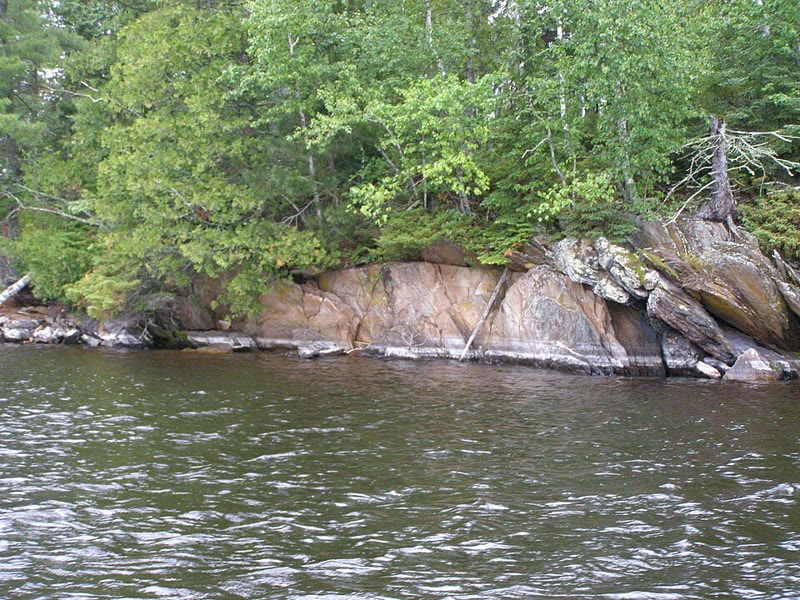
\includegraphics[height=5.0cm]{images/book2/g12-light-canadian-shield.jpg}

{\small Des gneiss et des granites vieux de 1 à 3~milliards d'années au
bord d'un lac du Canada, une partie du cœur ancien de l'Amérique du Nord.
Photographie Chris Light (CC~BY-SA~4.0).}
\end{omfigure}
% ledger: photo:g12-canadian-shield

Pourquoi la \omterm{def:g12:continental-crust:continental-crust}{croûte continentale} dure-t-elle, alors que le fond des océans
est toujours jeune~? La \omterm{def:g11:ocean-ridges:oceanic-lithosphere}{croûte océanique} est dense~: elle replonge dans le
manteau aux \omterm{def:g11:subduction-zones:subduction}{zones de subduction}, et aucune partie ne survit beaucoup plus
de 200 millions d'années. La \omterm{def:g12:continental-crust:continental-crust}{croûte continentale} est trop légère pour
s'enfoncer~; elle peut être usée par l'érosion, étirée ou plissée, mais
elle reste en surface. Les roches d'un continent sont une archive de quatre
milliards d'années.
% ledger: tulane:no-subduct, tulane:roots, data:b2-seafloor-age

\section{Les racines des montagnes}

Plus les montagnes sont hautes, plus la croûte est épaisse sous elles.

\begin{definition}[Racine d'une chaîne de montagnes]\label{def:g12:continental-crust:root}
La \emph{racine}\index{racine (d'une chaine de montagnes)@racine (d'une chaîne de montagnes)}
d'une chaîne de montagnes est la partie de sa croûte épaissie qui s'enfonce
dans le manteau au-dessous du niveau du \omterm{def:g11:seismic-structure:moho}{Moho} des plaines environnantes.
\end{definition}
% ledger: tulane:roots

Le modèle d'Airy prévoit la \omterm{def:g12:continental-crust:root}{racine}~: une chaîne qui domine ses environs de
$h$ a une \omterm{def:g12:continental-crust:root}{racine} $r = h\,\rho_c/(\rho_m - \rho_c)$, environ cinq fois sa
hauteur avec $\rho_c = \qty{2830}{kg/m^3}$ et
$\rho_m =
\qty{3380}{kg/m^3}$
(\cref{prop:g11:lithosphere-asthenosphere:airy}). Deux types de mesures
voient les \omterm{def:g12:continental-crust:root}{racines}. Les campagnes sismiques trouvent le \omterm{def:g11:seismic-structure:moho}{Moho} plus profond
sous les chaînes~: de 50 à \qty{70}{km} sous de nombreuses chaînes de
montagnes, environ \qty{70}{km} sous certaines parties du Tibet. La
pesanteur est plus faible au-dessus des chaînes de montagnes que ne le
laisserait penser leur masse visible~: la \omterm{def:g12:continental-crust:root}{racine} légère, qui tient la place
d'un manteau plus dense, crée un déficit de masse en profondeur, et les
anomalies de pesanteur mesurées suivent la topographie et l'épaisseur de la
croûte trouvée par la sismologie. Les continents flottent, et leurs
montagnes flottent plus haut encore.
% ledger: tulane:roots, karplus:tibet-moho, cm95:crust, data:prem

\section{Exercices}

\begin{exercise}[$\star$]\label{exo:g12:continental-crust:1}
Recopier et compléter pour la \omterm{def:g12:continental-crust:continental-crust}{croûte continentale} et la \omterm{def:g11:ocean-ridges:oceanic-lithosphere}{croûte
océanique}~: épaisseur~; principales roches~; teneur en silice~; masse
volumique~; âge maximal.
\end{exercise}

\begin{exercise}[$\star$]\label{exo:g12:continental-crust:2}
L'ensemble de la \omterm{def:g12:continental-crust:continental-crust}{croûte continentale} contient \qty{60.6}{\percent} de
silice, sa partie supérieure \qty{66.6}{\percent}. D'après les classes de
silice des roches magmatiques, chacune est-elle \omterm{def:g11:igneous-rocks:felsic-mafic}{mafique}, \omterm{def:g11:igneous-rocks:felsic-mafic}{intermédiaire} ou
\omterm{def:g11:igneous-rocks:felsic-mafic}{felsique}~? Nommer une \omterm{def:g11:igneous-rocks:volcanic-plutonic}{roche plutonique} de même composition.
\end{exercise}

\begin{exercise}[$\star$]\label{exo:g12:continental-crust:3}
Pourquoi la \omterm{def:g11:ocean-ridges:oceanic-lithosphere}{croûte océanique} peut-elle s'enfoncer dans le manteau à une
\omterm{def:g11:subduction-zones:subduction}{zone de subduction}, et pas la \omterm{def:g12:continental-crust:continental-crust}{croûte continentale}~? Répondre à l'aide des
masses volumiques.
\end{exercise}

\begin{exercise}[$\star$]\label{exo:g12:continental-crust:4}
(1) Qu'est-ce qu'un \omterm{def:g12:continental-crust:craton}{craton}~? (2) Quel âge ont au moins les roches d'un
\omterm{def:g12:continental-crust:craton}{craton}~? (3) Quels types de roches le constituent~?
\end{exercise}

\begin{exercise}[$\star$]\label{exo:g12:continental-crust:5}
Le plus ancien fond océanique a environ 190 millions d'années, le gneiss
d'Acasta 4.03~milliards d'années. Combien de fois le gneiss est-il plus
ancien~? Pourquoi n'y a-t-il pas de fond océanique aussi ancien~?
\end{exercise}

\begin{exercise}[$\star\star$]\label{exo:g12:continental-crust:6}
La \omterm{def:g12:continental-crust:continental-crust}{croûte continentale} couvre \num{210.4}~millions de~\unit{km^2}, dont
\qty{30.6}{\percent} sous la mer. (1) Quelle surface de \omterm{def:g12:continental-crust:continental-crust}{croûte continentale}
se trouve sous la mer~? (2) Quelle surface est émergée~? (3) La surface de
la Terre vaut $4\pi R^2$ avec $R = \qty{6371}{km}$. Quelle part de la
surface la \omterm{def:g12:continental-crust:continental-crust}{croûte continentale} couvre-t-elle~?
\end{exercise}

\begin{exercise}[$\star\star$]\label{exo:g12:continental-crust:7}
Calculer la masse d'une colonne de croûte de section \qty{1}{m^2}, de la
surface au \omterm{def:g11:seismic-structure:moho}{Moho}~: (1) à travers \qty{41.1}{km} de \omterm{def:g12:continental-crust:continental-crust}{croûte continentale} à
\qty{2830}{kg/m^3}~; (2) à travers \qty{7.1}{km} de \omterm{def:g11:ocean-ridges:oceanic-lithosphere}{croûte océanique} à
\qty{3000}{kg/m^3}. (3) Combien de fois la première est-elle plus
lourde~?
\end{exercise}

\begin{exercise}[$\star\star$]\label{exo:g12:continental-crust:8}
Une chaîne domine de \qty{2.5}{km} des plaines dont la croûte est épaisse
de \qty{35}{km}. Avec $\rho_c = \qty{2830}{kg/m^3}$ et
$\rho_m =
\qty{3380}{kg/m^3}$, calculer sa \omterm{def:g12:continental-crust:root}{racine} et l'épaisseur de sa
croûte. Le résultat est-il dans l'intervalle mesuré sous les chaînes de
montagnes~?
\end{exercise}

\begin{exercise}[$\star\star$]\label{exo:g12:continental-crust:9}
D'après l'histogramme des âges du fond océanique~: (1) quelle part du fond
océanique a moins de 30 millions d'années~? (2) Quelle tranche de 10
millions d'années contient le plus de fond~? (3) Pourquoi la part
diminue-t-elle vers les âges anciens~?
\end{exercise}

\begin{exercise}[$\star\star$]\label{exo:g12:continental-crust:10}
Cartographiée avec ses parties immergées, la \omterm{def:g12:continental-crust:continental-crust}{croûte continentale} a une
altitude moyenne d'environ \qty{120}{m}. Supposer que ses parties
immergées, \qty{30.6}{\percent} de sa surface, se trouvent en moyenne à
\qty{100}{m} sous le niveau de la mer. Quelle est l'altitude moyenne de sa
partie émergée~? Pourquoi les estimations plus anciennes, qui ne comptaient
que les terres émergées, donnent-elles une altitude moyenne bien plus
élevée~?
\end{exercise}

\begin{exercise}[$\star\star$]\label{exo:g12:continental-crust:11}
Un forage sur une île située loin au milieu d'un océan atteint, sous
quelques centaines de mètres de laves, un \omterm{def:g11:ocean-ridges:gabbro}{gabbro}~; les profils sismiques
placent le \omterm{def:g11:seismic-structure:moho}{Moho} à \qty{8}{km} de profondeur. Un autre forage, sous une
vaste plaine plate, atteint du gneiss à \qty{2}{km}, et le \omterm{def:g11:seismic-structure:moho}{Moho} se trouve à
\qty{38}{km} de profondeur. Utiliser la méthode pour décider quelle croûte
se trouve sous chacun.
\end{exercise}

\begin{exercise}[$\star\star\star$]\label{exo:g12:continental-crust:12}
Quelle est la qualité de l'approximation de la proposition~? (1) Calculer
le volume exact d'une coquille d'épaisseur \qty{41.1}{km} à la surface
d'une sphère de rayon \qty{6371}{km},
$\tfrac{4}{3}\pi\bigl(R^3 - (R - H)^3\bigr)$, et le volume approché,
$4\pi R^2 H$. (2) Quel est l'écart relatif~? Le comparer à $H/R$.
\end{exercise}

\begin{exercise}[$\star\star\star$]\label{exo:g12:continental-crust:13}
Supposer que le tiers supérieur de la \omterm{def:g12:continental-crust:continental-crust}{croûte continentale}, en masse,
contient \qty{66.6}{\percent} de silice, et la croûte entière
\qty{60.6}{\percent}. (1) Quelle est la teneur en silice des deux tiers
inférieurs~? (2) À quelle classe de roches magmatiques correspond-elle~?
(3) Qu'est-ce que cela dit de la \omterm{def:g12:continental-crust:continental-crust}{croûte continentale} profonde~?
\end{exercise}

\begin{exercise}[$\star\star\star$]\label{exo:g12:continental-crust:14}
Supposer que de la \omterm{def:g11:ocean-ridges:oceanic-lithosphere}{croûte océanique} nouvelle se forme aux dorsales à
raison d'environ \qty{3}{km^2} par an, et que le fond océanique couvre
environ \num{300}~millions de~\unit{km^2}. (1) Combien de temps les
dorsales mettraient-elles à fabriquer une surface égale à celle de tout le
fond océanique~? (2) Comparer aux âges du fond océanique. (3) Que doit-il
arriver à l'ancien fond~?
\end{exercise}

\begin{exercise}[$\star\star\star$]\label{exo:g12:continental-crust:15}
Supposer que toute la \omterm{def:g12:continental-crust:continental-crust}{croûte continentale}, \qty{8.6e9}{km^3}, s'est formée
à un rythme constant depuis 4.0~milliards d'années. (1) Calculer ce rythme
en kilomètres cubes par an. (2) Les zircons des Jack Hills montrent qu'une
croûte existait déjà il y a 4.4~milliards d'années. Un rythme constant
convient-il à un monde où la plus grande partie de la croûte se serait
formée tôt, ou tard~? Que peuvent dire les roches les plus anciennes, et
que ne peuvent-elles pas dire, sachant qu'une croûte ancienne peut être
érodée ou recyclée~?
\end{exercise}

\section{Problème~: quelle est la masse de la croûte continentale~?}

\begin{problem}[{Problème du week-end --- la masse des continents}]
\label{pb:g12:continental-crust:1}
% ledger: cogley84:continents, cm95:crust, earth:mass, earth:Rmean, earth:density, white92:crust
% values: 4 pi R^2 = 5.1006e8 km2; V = 210.4e6 x 41.1 = 8.647e9 km3; m = 2.447e22 kg; m/M = 0.410 %
La \omterm{def:g12:continental-crust:continental-crust}{croûte continentale} couvre \num{210.4}~millions de~\unit{km^2} (parties
immergées comprises). Les campagnes sismiques lui donnent une épaisseur
moyenne de \qty{41.1}{km} et une masse volumique moyenne de
\qty{2830}{kg/m^3}. La Terre a un rayon moyen de \qty{6371}{km}, une masse
de \qty{5.9722e24}{kg} et une masse volumique moyenne de
\qty{5513}{kg/m^3}.

\medskip
\noindent\textbf{Partie I --- La surface.}
\begin{enumerate}
  \item Calculer l'aire de la surface de la Terre, $4\pi R^2$, en
        \unit{km^2}.
  \item Quelle part en couvre la \omterm{def:g12:continental-crust:continental-crust}{croûte continentale}~?
  \item \qty{30.6}{\percent} de la \omterm{def:g12:continental-crust:continental-crust}{croûte continentale} se trouve sous la
        mer. Quelle surface cela représente-t-il~?
  \item Quelle surface de la Terre reste-t-il pour la \omterm{def:g11:ocean-ridges:oceanic-lithosphere}{croûte océanique}, en
        supposant que tout le reste est océanique~?
  \item Pourquoi la \omterm{def:g12:continental-crust:continental-crust}{croûte continentale} est-elle plus étendue que les terres
        émergées~?
\end{enumerate}

\medskip
\noindent\textbf{Partie II --- Épaisseur et volume.}
\begin{enumerate}[resume]
  \item Pourquoi peut-on calculer le volume comme l'aire multipliée par
        l'épaisseur, alors que la croûte repose sur une sphère~?
  \item Calculer le volume de la \omterm{def:g12:continental-crust:continental-crust}{croûte continentale} en \unit{km^3}.
  \item Le convertir en \unit{m^3}.
  \item Une autre estimation de l'épaisseur moyenne donne \qty{36}{km}.
        Quel volume en résulte-t-il~?
  \item De combien, en pourcentage, les deux volumes diffèrent-ils~?
\end{enumerate}

\medskip
\noindent\textbf{Partie III --- Masse volumique et masse.}
\begin{enumerate}[resume]
  \item Calculer la masse de la \omterm{def:g12:continental-crust:continental-crust}{croûte continentale} avec \qty{41.1}{km}.
  \item Calculer la masse d'une colonne de \qty{1}{m^2} à travers la \omterm{def:g12:continental-crust:continental-crust}{croûte
        continentale}.
  \item Calculer la masse de la \omterm{def:g11:ocean-ridges:oceanic-lithosphere}{croûte océanique}~: surface de la
        question~4, épaisseur \qty{7.1}{km}, masse volumique
        \qty{3000}{kg/m^3}.
  \item Laquelle est la plus lourde, et combien de fois~? Pourquoi, alors
        qu'elle couvre une moindre surface~?
  \item Pourquoi la \omterm{def:g12:continental-crust:continental-crust}{croûte continentale} est-elle moins dense que la \omterm{def:g11:ocean-ridges:oceanic-lithosphere}{croûte
        océanique}~?
\end{enumerate}

\medskip
\noindent\textbf{Partie IV --- Comparée à la Terre.}
\begin{enumerate}[resume]
  \item Diviser la masse de la question~11 par la masse de la Terre.
  \item Vérifier le résultat à l'aide de la proposition sur les couches
        minces.
  \item Quelle part de la masse de la Terre la \omterm{def:g11:ocean-ridges:oceanic-lithosphere}{croûte océanique}
        représente-t-elle~?
  \item La \omterm{def:g12:continental-crust:continental-crust}{croûte continentale} contient les seules roches de plus de 200
        millions d'années environ. Quelle part de la masse de la Terre porte
        l'archive de presque toute son histoire~?
  \item Conclure~: quelle part de la masse de la Terre la \omterm{def:g12:continental-crust:continental-crust}{croûte
        continentale} représente-t-elle~?
\end{enumerate}
\end{problem}
